%%%%%%%%%%%%%%%%%%%%%%%%%%%%%%%%%%%%%%%%%%%%%%%%%%%%
%    Canadian AI Latex Template    %
%%%%%%%%%%%%%%%%%%%%%%%%%%%%%%%%%%%%%%%%%%%%%%%%%%%%

\documentclass[10pt]{cai}

% Graphics should all go in the figs/ directory
\graphicspath{{figs/}}


\begin{document}

% Editorial staff will replace the following values:
% 1. Conference Year
% 2. Issue number
% 3. Article DOI
\volumeheader{36}{0}%{00.000}
\begin{center}

  \title{Image Captioning Dataset in Persian Using Flicker30k Images}
  \maketitle

  \thispagestyle{empty}

  % Add Authors and Affiliations in the camera ready
  % for the double blind review, please leave this section as is 
  \begin{tabular}{cc}
    Shima Baniadamdizaj\upstairs{\affilone}, Alexander Breuer\upstairs{\affilone}
   \\[0.25ex]
   {\small \upstairs{\affilone} Fredrich Schiller University Jena} \\
  \end{tabular}
  
  % Replace with corresponding author email address
  \emails{
    \upstairs{*}corresponding\_author@example.ca 
    }
  \vspace*{0.2in}
\end{center}

\begin{abstract}

The 36th Canadian Conference on Artificial Intelligence (Canadian AI 2023) will take place physically in Montreal, from June 5 to 9, 2023. The event is collocated with the Computer and Robot Vision (CRV) conference. These events (AI-CRV 2023) will bring together hundreds of leaders in research, industry, and government, as well as Canada's most accomplished students. They showcase Canada's ingenuity, innovation and leadership in intelligent systems and advanced information and communications technology.\\
\end{abstract}

% add your keywords
\begin{keywords}{Keywords:}
keyword1, keyword2, keyword3, up to 6
\end{keywords}
\copyrightnotice

\section{Introduction}
\label{intro}
We invite papers that present original work in all areas of Artificial Intelligence, either theoretical or applied. Canadian AI 2023 welcomes submissions on topics including (but not limited to):
\begin{figure}[H]
    \centering
    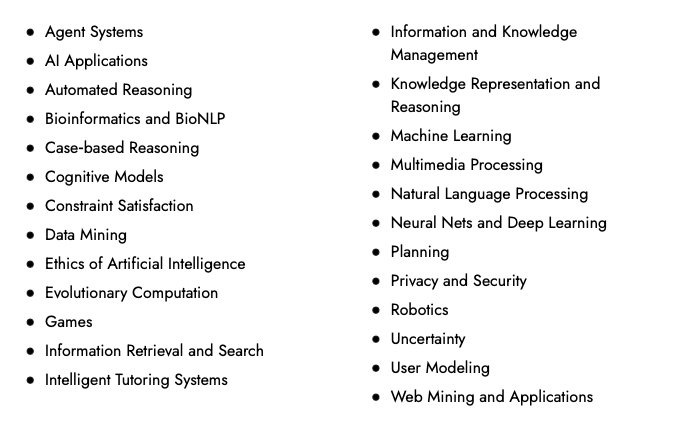
\includegraphics[scale=0.6]{figs/sample_fig.png} \\
    \caption{List of topics (but not limited to)}
    \label{fig:sample_fig}
\end{figure}
\
We expressly encourage work that cuts across technical areas or applies AI techniques in the context of important domains such as e-commerce, games, healthcare, sustainability,  transportation, Internet of Things, and agriculture.

Moreover, we plan to have a collocated event on Ethics of AI, with a joint invited keynote and other activities related to this topic. We therefore encourage papers highlighting research in this specific area.

We also welcome the submission of position papers, which present evidence-based arguments for a particular point of view without necessarily presenting a new system. There will be an option during the submission process to indicate that a paper is a position paper.

\subsection{Important Dates}
\label{important}

\begin{table}[h]
\begin{tabular}{ |l|l| }
 Submission deadline: & February 12th, 2023 (11:59 p.m. UTC-12) \\ 
 Author notification: & March 26th, 2023 \\  
 Final papers due: & April 9th, 2023 \\
 Main conference: & June 5 to 9, 2023
\end{tabular}
\vspace{0.2cm}
\caption{Important dates}
\label{tab:important}
\end{table}

\section{Submission Details}
\label{submission}
We invite submissions of both long and short papers. Long papers must be no longer than \textbf{12 pages}, and Short papers must be no longer than \textbf{6 pages}, including references, formatted using the conference template. The authors should consult the authors guidelines and use the provided proceedings template to prepare their papers  \cite{cai2020,author1_name_author_2020}.

Papers submitted to the conference must not have already been published, or accepted for publication, or be under review by a journal or another conference. Submissions will go through a \textbf{double-blind} review process by Program Committee members to assess originality, significance, technical merit, and clarity of presentation. As such, submissions must be anonymized, and papers that fail to do so will be rejected without review.  A “Best Paper Award” and a “Best Student Paper Award” will be given at the conference respectively to the authors of each best paper, as judged by the Best Paper Award Selection Committee.

\section{Publication}
\label{pub}

The conference proceedings will be published in PubPub open access online format \cite{pubpub2020}, and submitted to be indexed/abstracted in leading indexing services such as DBLP, ACM, Google Scholar. A paper will be accepted either as a long or as a short paper. Long papers will be allocated 12 pages while short papers will be allocated 6 pages in the proceedings. Authors of accepted papers will be allocated time for an oral presentation at the conference and will have the opportunity to present their work in a poster session. 

At least one author of each accepted paper is required to attend the conference to present the work. The authors must agree to this requirement prior to submitting their paper for review.

In addition, the corresponding author of each paper, acting on behalf of all of the authors of that paper, must complete and sign a Consent-to-Publish form. The corresponding author signing the copyright form should match the corresponding author marked on the paper.

\section*{Acknowledgements}
Canadian AI is sponsored by the Canadian Artificial Intelligence Association(CAIAC)\cite{caiac}.

%Begin appendix section(s)
\appendix

% Add appendices here:
\section{Example of math equation }
%\label{appendix-customize-this-label}
Binomial theorem: \cite{abramowitz1948handbook}
\begin{equation}
(x+y)^n=\sum_{\substack{k=0}}^{n}\dbinom{n}{k}x^{n-k}y^k
\end{equation}




% All references should be stored in the file "references.bib"
% Please do not modify anything below this line.
%\thispagestyle{plain}
%\printbibliography

\printbibliography[heading=subbibintoc]

\end{document}
